
\documentclass[twoside, twocolumn]{ctexart}

\usepackage[top=2.54cm, bottom=2.54cm, left=3.18cm, right=3.18cm]{geometry}
\usepackage[colorlinks, linkcolor=blue]{hyperref}
\usepackage{balance, fancyhdr}
\usepackage[perpage]{footmisc}
\usepackage{titlesec, caption}
\usepackage{amsmath, xfrac, upgreek}
\usepackage{amsthm}
\usepackage{fontspec, txfonts, pifont}
\usepackage{tikz, tkz-euclide}
\usepackage{graphicx, incgraph}
\usepackage[x11names]{xcolor}
\usepackage{booktabs, multirow, array}

\pagestyle{fancy}
\fancyhead[RO,LE]{\thepage} \fancyfoot[C]{}
\fancyfoot[LE]{\small
  Copyright \copyright\ 2024 \textbf{Liu One}
  \quad \emph{All rights reserved.}}
\fancyfoot[RO]{\small\textit{版权所有,侵权必究。}}
\setlength{\headheight}{12.64723pt}
\addtolength{\topmargin}{-0.64723pt}

\titleformat{\section}{\bfseries}{总第\thesection 题}{.5em}{\LARGE\ttfamily}
\titleformat{\subsection}{\large\bfseries}{方法\chinese{subsection}:}{0pt}{\itshape}
\titleformat{\subsubsection}{\bfseries}{第\chinese{subsubsection}步}{.5em}{}

\renewcommand\thefootnote{\ding{\numexpr171+\value{footnote}}}

\setmainfont{Times New Roman}
\setsansfont{Helvetica}
\setmonofont{Courier New}
\setCJKmainfont[
  BoldFont={黑体-简 中等}, ItalicFont={楷体-简},
  BoldItalicFont={宋体-简 黑体}]{宋体-简}
\setCJKsansfont{黑体-简}
\setCJKmonofont[BoldFont=华文仿宋]{华文仿宋}

\allowdisplaybreaks
\numberwithin{equation}{section}
\newtheorem{lemma}{引理}[section]

\captionsetup{format=hang, font=small, labelfont=bf, labelsep=quad}

\columnsep=3em
\columnseprule=0.5pt

\usetikzlibrary{
  angles, quotes, calc, intersections, through, shadows,
  decorations.pathmorphing}
\tikzset{
  mark angle/.style n args={3}{
    draw=#1!50, fill=#1!20,
    angle radius=#2, angle eccentricity=#3,
  },
  opafill/.style n args={1}{
    fill=#1!50, fill opacity=.5,
  },
}

\setcounter{tocdepth}{2}
\newcommand\prob[2]{\section{#1\normalsize\ #2} \label{sec:#1}}
\newcommand\ans[1]{\noindent\hrulefill\\\textbf{答案}\quad#1\hfill}
\newcommand\problabels[2][]{
  \hfill \foreach \labelcolor/\labelname in {#2} {
    \tikz[baseline=($ (label.center)!1/2!(label.south) $)]
      \node[draw, rectangle, rounded corners=3pt,
        fill=\labelcolor!20, inner sep=2pt,
        minimum height=13pt, #1] (label) {
          \footnotesize\textit{\labelname}}; } }
\newcommand\image[1]{\input{images/#1}}
\newcommand\mathalignsep{\hspace{13pt}}

\let\oldcong\cong \let\oldsim\sim
\renewcommand\cong{\ \reflectbox{$\oldcong$}\ }
\renewcommand\sim{\ \reflectbox{$\oldsim$}\ }
\DeclareMathOperator\dif{d\!}
\renewcommand\pi{\uppi}
\newcommand\mathe{\mathrm{e}}
\newcommand\mathi{\mathrm{i}}
\newcommand\lcm{\mathrm{lcm}}
\newcommand\rttri{\mathrm{Rt}\triangle}

\newcommand\calclen[4]{sqrt((#1-#3)^2+(#2-#4)^2)}
\newcommand\calcdotpos[3]{(#1+#3*(#2-#1))}
\newcommand\calcbisectorx[6]{\calcdotpos#1#5{
  \calclen#1#2#3#4/(\calclen#1#2#3#4+\calclen#3#4#5#6)}}
\newcommand\calcbisectory[6]{\calcdotpos#2#6{
  \calclen#1#2#3#4/(\calclen#1#2#3#4+\calclen#3#4#5#6)}}

\setcounter{section}{128}
\includeonly{probs/00B7}
\title{\textbf{Liu One的数学题集}(\textit{VOL. 3}\quad 0080 -- 00BF)}
\author{Copyright \copyright\ 2024 \textbf{Liu One}
  \quad \emph{All rights reserved.} \\
  \textit{版权所有,侵权必究。}}
\date{}

\begin{document}

  
\onecolumn
\begin{inctext}[paper=graphics]
  \begin{tikzpicture}
    \coordinate (below left) at (0in,0in);
    \coordinate (above right) at (8.5in,11in);
    \path[use as bounding box] (below left) rectangle (above right);
    \draw[very thin, Seashell2] (below left) grid (above right);
    \draw (0,25) node[right]
      {\fontsize{100pt}{0pt}\selectfont
        \textbf{Math\textit{\textcolor{DodgerBlue2}{P}}robs}};
    \foreach \pos/\char in {21/数,17.5/学,14/题,10.5/集} {
      \draw (0,\pos) node[right]
        {\fontsize{100pt}{0pt}\selectfont \textbf{\textit{\char}}}; }
    \fill[DeepSkyBlue2] (17.5,23.9) rectangle (22,25.5);
    \fill[DarkSlateGray3] (10,0) -| (22,8) -- cycle;
    \draw (21.5,3) node[left]
      {\fontsize{60pt}{0pt}\selectfont
      \textcolor{DarkSlateGray1}{\textbf{\texttt{0080}}}};
    \draw (21.5,1) node[left]
      {\fontsize{60pt}{0pt}\selectfont
      \textcolor{DarkSlateGray1}{\textbf{-- \texttt{00BF}}}};
    \draw (17.5,24.7) node[right] {
      \begin{minipage}{10cm}
        \fontsize{10pt}{10pt}\selectfont \textcolor{Azure1}
        {Copyright \copyright\ 2024 \\
          \textbf{Liu One} \\ \emph{All rights reserved.}}
      \end{minipage} };
    \draw (0,6.9) node[right] {
\includegraphics[scale=.45]{covers/logo}};
    \draw (2,4) node {\Huge\textcolor{RoyalBlue1}{\textbf{VOL.}}};
    \draw (2,2) node
      {\fontsize{100pt}{0pt}\selectfont\textcolor{RoyalBlue2}{\textbf{3}}};
    \draw (13,6) node {
      \begin{minipage}{3cm}
        \footnotesize \textit{
        \raggedright 质数螺旋 \\
        \raggedleft ——混沌中的秩序 \\ }
      \end{minipage} };
    \begin{scope}[shift={(12,15)}, scale=.9, very thick]
      \draw (0,0) node {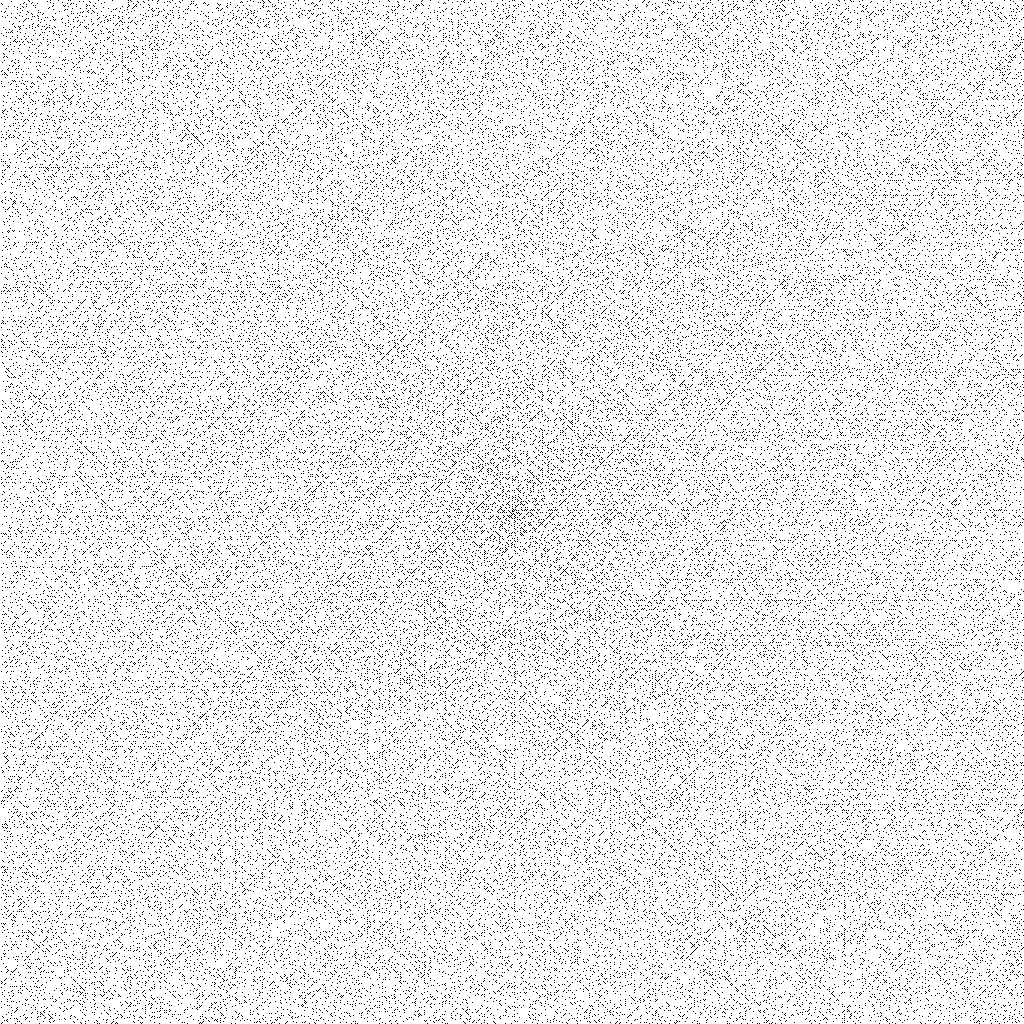
\includegraphics[width=16cm]{images/primes}};
    \end{scope}
  \end{tikzpicture}
\end{inctext}
\twocolumn

  \balance
  \maketitle
  \tableofcontents

  \foreach \probno in {
    0080, 0081, 0082, 0083, 0084, 0085, 0086, 0087,
    0088, 0089, 008A, 008B, 008C, 008D, 008E, 008F,
    0090, 0091, 0092, 0093, 0094, 0095, 0096, 0097,
    0098, 0099, 009A, 009B, 009C, 009D, 009E, 009F,
    00A0, 00A1, 00A2, 00A3, 00A4, 00A5, 00A6, 00A7,
    00A8, 00A9, 00AA, 00AB, 00AC, 00AD, 00AE, 00AF,
    00B0, 00B1, 00B2, 00B3, 00B4, 00B5, 00B6, 00B7
  } { \include{probs/\probno} }

\end{document}
